
\chapter{State of the Art}
\label{Chapter2}

In this chapter we present some of the tools which had a big impact in the field of bioinformatics, and especially metagenomics. Even though we focus on abundance estimation techniques, we provide an overview of the most important methods for the assignment of reads, both based on alignments and on $k$-mer composition, since their properties highly influenced the solutions adopted for the estimation of abundances. This list is not nearly extensive, and we refer to \cite{kucherov_algorithms_2018} for a more detailed overview of advances in bioinformatics, and to \cite{brinda_novel_2016} for an extensive list of tools.

\section{Read Mapping}
\subsection{Alignment-based Methods}
\begin{itemize}
    \item \textbf{BLAST} \cite{altschul_basic_1990}: developed in 1990, this is the first alignment method to be used in practice for metagenomics, namely in the notorious framework MEGAN \cite{huson_megan_2007}. Compared to the previous methods solely based on dynamic programming, whose output is the optimal alignment of two sequences (according to some parameters and to the definition of optimality, based on matches, mismatches, insertions and deletions in the alignment), this tool uses heuristics to achieve orders of magnitude higher alignment speed. The way it works is according to the \textit{seed-and-extend} paradigm: first, a subsequence of the read to align is queried in an index containing informative subsequences of the reference genomes (\textit{seeding} step), then if an exact match is found the program extends it using an alignment algorithm (\textit{extending} step). If the alignment score drops below a certain threshold, the alignment is interrupted and another seed is used. This last optimization has a huge drawback when the reads come from a metagenome: in the presence of a novel organism which is not included in the reference database, BLAST will stop the query reporting no alignment, decreasing the overall sensitivity of the method. A desirable property of aligners for metagenomics would be to report even low-quality alignments with genomes similar to the query, which can still provide useful information on the composition (especially if the references are organized in a taxonomic tree). Even though the threshold can theoretically be reduced, the trade-off between sensitivity and time complexity often leads to unsatisfactory results. Furthermore, the use of an extensive reference database requires TBs of memory to store the huge hash table used to store the seeds. Even though several other alignment algorithms have been developed during the 90's and the beginning of this century, BLAST has been keeping to attract users till nowadays: it and its numerous optimizations are still used extensively in various scenarios, including metagenomics.
    \item \textbf{BWA-MEM} \cite{li_aligning_2013}: one of the most used alternatives to BLAST is currently BWA framework's aligner BWA-MEM. The algorithm is based on identifying maximum exact matches (MEM) between the suffixes of the read and the reference sequences. Those matches are used as seeds and extended similarly to what is done in BLAST. The main innovation brought by this tool is the use of an efficient indexing structure, the BWT-index. This data structure, first introduced for full-text search applications, makes use of a reversible text permutation, the Burrows-Wheeler transform, which reduces the entropy of the sequence to be indexed by grouping runs of the same characters. While this is especially useful for compression, it also has a deep relationship with suffix arrays and, thanks to an additional data structure, it allows for queries of a pattern of length $p$ occurring $occ$ times in the reference in time $\mathcal{O}(p+occ)$. This efficient index has become a mainstream data structure in bioinformatics, and several other tools are based on it. In addition to being very memory efficient, BWA is also much faster than BLAST: aligning 1M reads to the first 9 chromosomes of the human genome, for instance, takes BWA only 6 minutes, while BLAST requires more than 24 hours.
\end{itemize}
\subsection{Alignment-free Methods}
\begin{itemize}
    \item \textbf{Kraken} \cite{wood_kraken:_2014}: this is among the first alignment-free tools developed for metagenomic classification, and it set a new standard for assignment speed, allowing to analyze up to one million metagenomic reads per CPU minute. In addition to the set of reference sequences, Kraken uses the taxonomic tree on which they are clustered to compress the database and speed up the queries. Its index consists of a hash table associating each $k$-mer to the lowest common ancestor (LCA) of the reference genomes containing it in the taxonomic tree. This data structure provides very fast queries, but requires large amounts of memory. Furthermore, the LCA statistics requires a fundamental assumption to be verified by the tree topology: a k-mer associated to an internal node should be present in most reference genomes of its subtree. This is far from being true, because of phenomena like horizontal gene transfer which allows bacteria of different species to ``exchange'' portions of their genomes, and because taxonomic trees are built not only upon actual sequence similarity, but also on morphology, history and geography of their discovery, harmness to humans etc. As a consequence, propagating a $k$-mer present in only two genomes which are very distant in the tree to its LCA introduces a considerable number of false positives, since in the database this $k$-mer will be considered as present in every genome in the subtree of the LCA. In conclusion, even though Kraken has opened new possibilities in metagenomics thanks to its classification speed, its applications are now limited because of the amount of memory it requires and the LCA heuristics getting less and less accurate as more genomes are sequenced and included in the reference databases. As explored in \cite{nasko_refseq_2018}, at the current state the NCBI RefSeq database requires 2TB of memory and 11 days to be indexed by Kraken, and while the percentage of classified sequences increases considerably with the expansion of the database, the overall accuracy of the method decreases, most likely because of flaws in the LCA assumption when tens of thousands of reference genomes are indexed.
    \item \textbf{ProPhyle} \cite{brinda_prophyle:_2017}: addressing the main issues in Kraken and its legacy, ProPhyle moves forward from the LCA heuristics to a lossless index where each $k$-mer is associated to the exact set of genomes where it appears. In doing so, it surprisingly reduces the amount of memory required both for the creation of the index and the classification of sequences with respect to Kraken. The same reference database, containing around 2700 bacterial genomes, which would require 90GB of memory for the construction of a Kraken database and 70GB for the classification of reads, will only require under 16GB with ProPhyle, fitting a laptop's resources. This program propagates $k$-mers up in the taxonomic tree only if they are shared by every child of a given node, and compresses the set of $k$-mers associated with a node using an assembly algorithm based on the greedy enumeration of disjoint paths in a De-Bruijn graph. While this process enables the compression of the $k$-mer information required from the reference sequences, the topology of the tree only plays a role in defining the compression rate and the speed of the classifier, but not on its accuracy; furthermore, the choice is not limited to commonly used taxonomic trees as the NCBI one used by Kraken, but any phylogenetic tree in the Newick format can be used. The collection of sequences resulting from this compression process is indexed using the BTW-index, providing slightly slower queries than Kraken but considerably reducing the memory requirements while providing more accurate assignments as shown in figure \ref{fig:mult_ass}. In particular, reads matching several nodes with the same score are assigned to the entire set, and the output contains the exact information about each $k$-mer match and mismatch for every node.
\end{itemize}

\begin{sidewaysfigure}
  \caption{Average assignment sets cardinalities for ProPhyle, Kraken and Centrifuge. The index for the tree tools were built from a set of 50 genomes from each of the 25 species listed in the $x$-axis, for a total of 1250 genomes. Reads were simulated from each genome and assigned to the index. On the $y$-axis is the average size of a read's assignment set (number of genomes in the subtrees when assignments are to internal nodes). ProPhyle's assignments are more specific than those of the other tools, making it a better candidate for metagenomic classification with indexes including several thousands of similar reference genomes.}
  \centering
    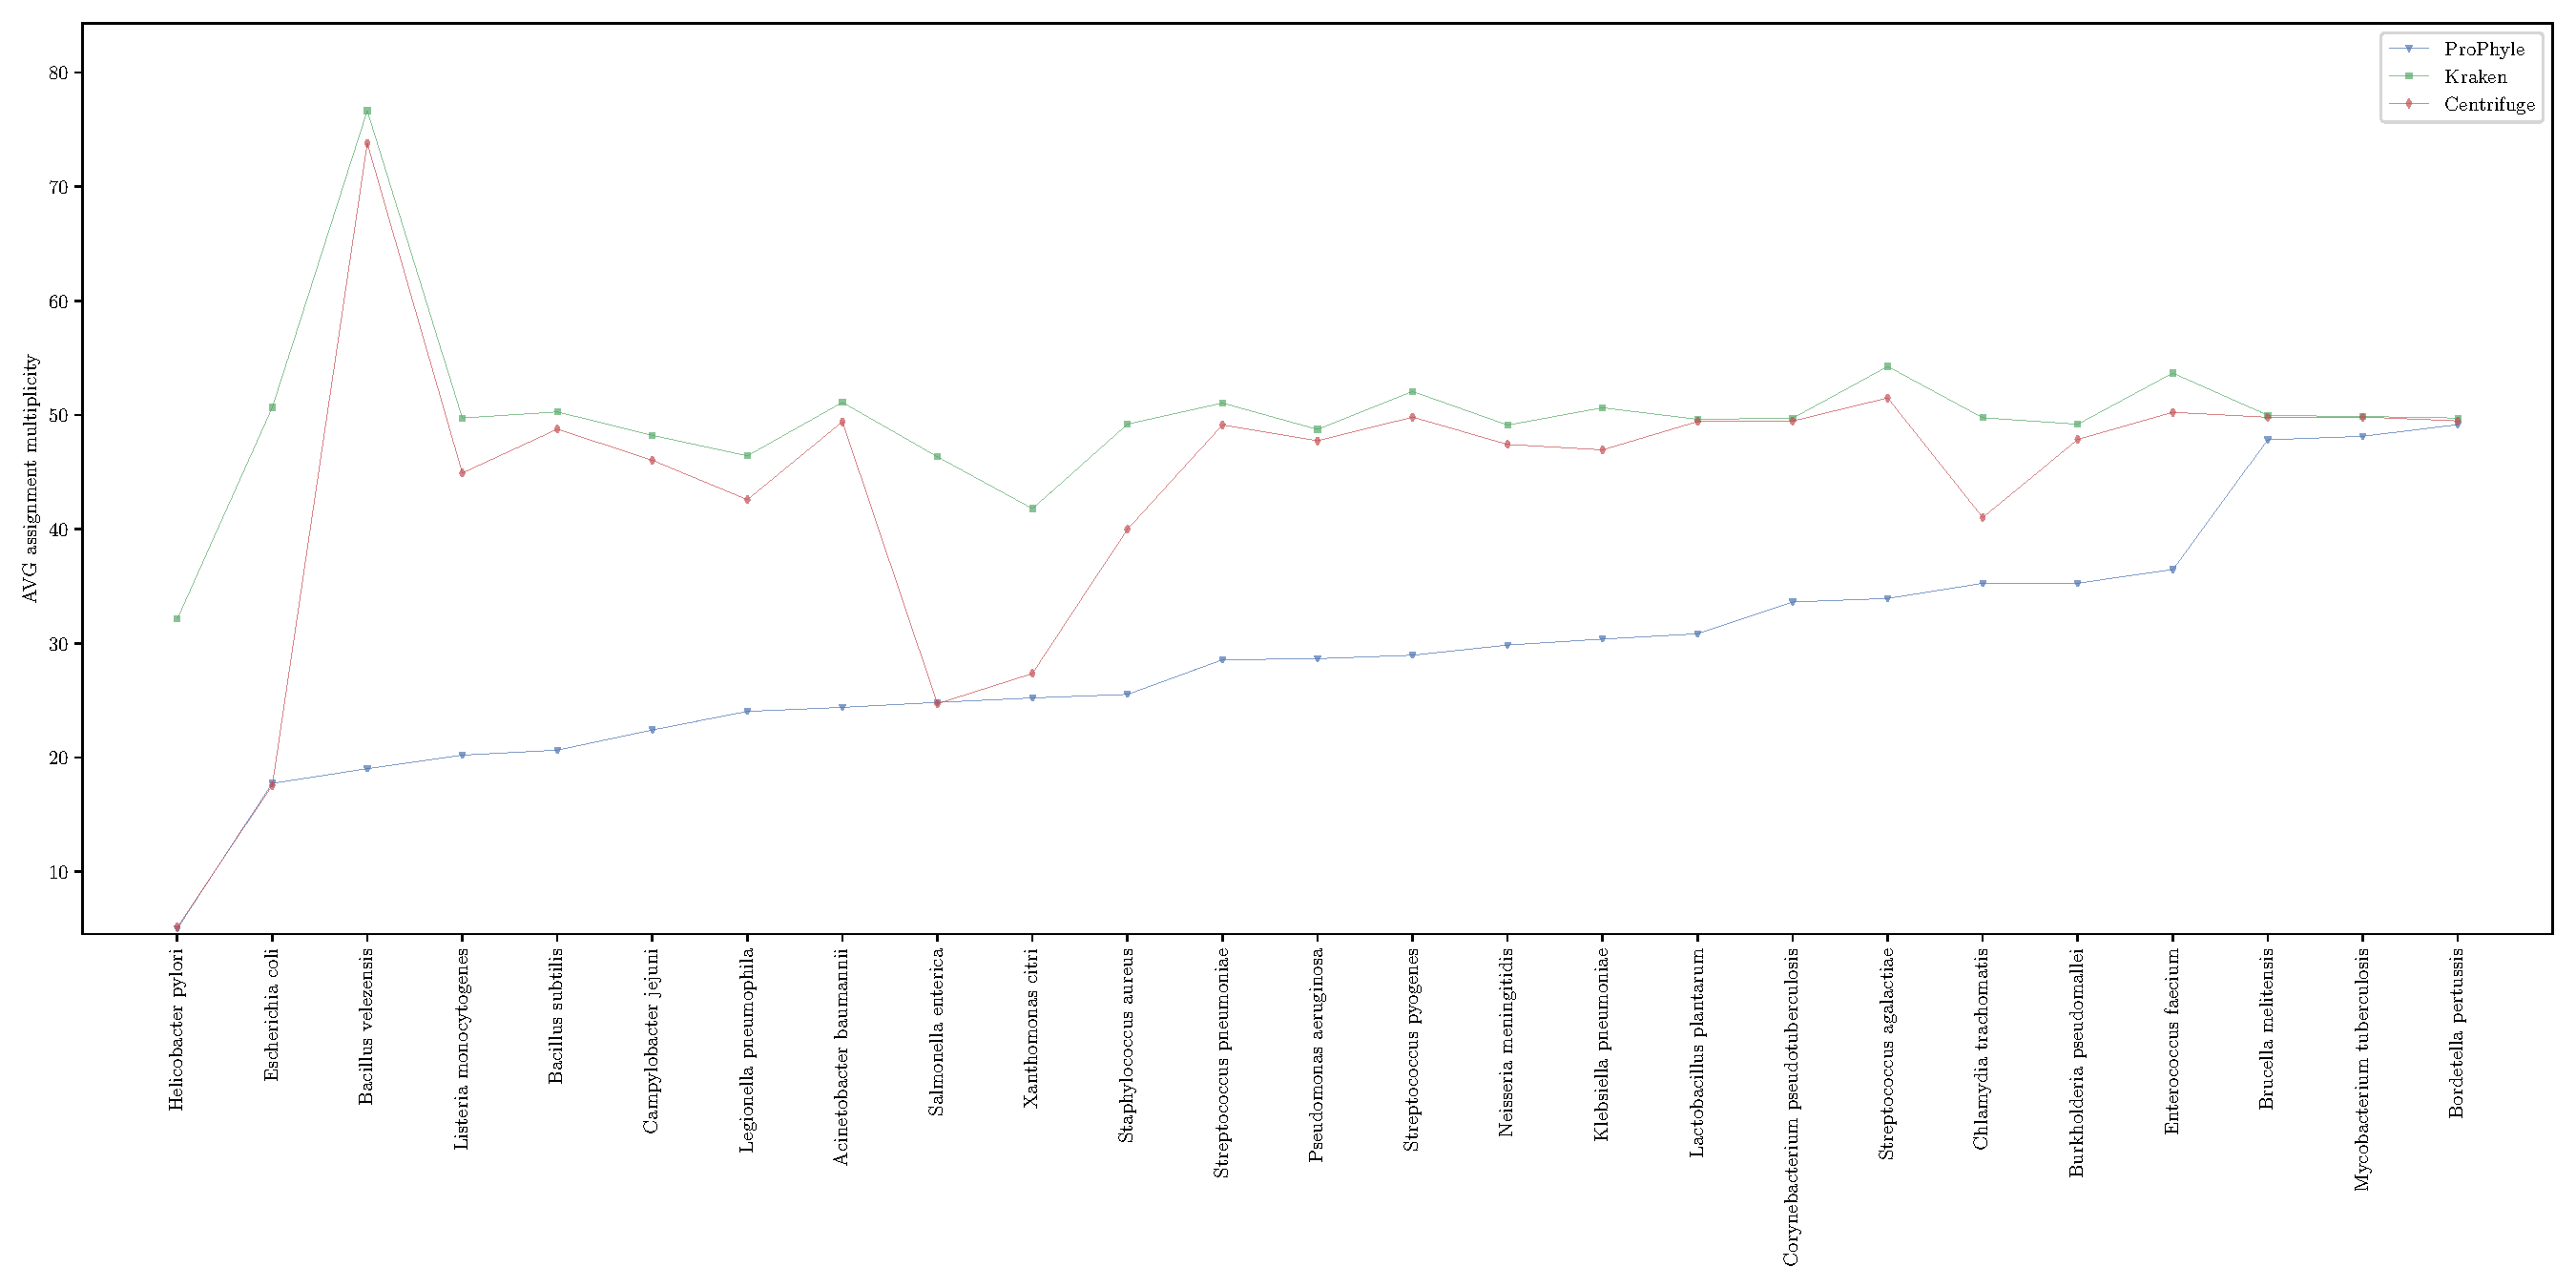
\includegraphics[width=1\textwidth]{Figures/mult_ass.pdf}
  \label{fig:mult_ass}
\end{sidewaysfigure}

\section{Abundance Estimation}

\subsection{Bayesian Re-estimation}
\begin{itemize}
    \item \textbf{Bracken} \cite{lu_bracken:_2017}: the purpose of this tool, whose name stands for Bayesian Reestimation of Abundance after Classification with KrakEN, is to reduce the bias due to the lossy database of Kraken by estimating the probability that reads from a reference genome are assigned to its ancestors in the taxonomic tree. Using Bayes' theorem, this information is inversed to estimate the probability that a read assigned to an internal node comes from the leaves (genomes) in its subtree, enabling the re-distribution of those reads to the genomes. In the publication, the authors show that the tool is able to achieve a satisfying estimation of abundances of two notoriously complex species, Mycobacterium Bovis and Mycobacterium Tuberculosis, whose genomes are characterized by >99.5\% similarity. Nevertheless, this approach has a main drawback: it introduces a vast number of false positives by redistributing reads assigned to internal nodes to genomes which were not in the sample in the first place; even though users can specify a threshold for the minimum number of specific assignments that a genome needs to have to be considered as present in the sample, this does not allow to correctly filter false positives because of the combination of the LCA heuristic and biases in the representation of different species, where some have thousands of representative genomes and therefore it is less likely to have specific assignment to a single one, while others have only one representative.
\end{itemize}

\subsection{Expectation-Maximization}
\begin{itemize}
    \item \textbf{Kallisto} \cite{bray_near-optimal_2016}: born as a RNA-seq quantification program, Kallisto has been applied to metagenomics in its variant Metakallisto. After assigning reads to equivalence classes, i.e. set of reference genomes likely to have generated them computed by intersecting the $k$-equivalent classes of each $k$-mer they are composed of, Kallisto runs an Expectation Maximization (EM) algorithm, inherited by its predecessors Cufflinks and Sailfish, to estimate the real abundances from the counts of assignments to equivalence classes. The EM algorithm iteratively optimizes the likelihood of parameters in a statistical model. It alternates between two steps: in the E-step it calculates the likelihood with the current parameters, and in the M-step it sets the parameters to maximize its value. An example of definition of such model is given for Centrifuge.
    \item \textbf{Centrifuge} \cite{kim_centrifuge:_2016}: the EM algorithm applied to RNA-seq quantification influenced several other metagenomic classifiers, including MetaMaps \cite{dilthey_metamaps_2018} and Centrifuge. This tool is based on the BWT-index and on probabilistic propagation of subsequences of the reference genomes in a taxonomic tree, and computes pseudoalignments with an heuristic seed-and-extend algorithm. Starting from these pseudoalignments, the likelihood of an abundance vector at i.e. the species level is defined as follows:
    \begin{equation*}
      L(\alpha|C) = \prod_{i=1}^R \sum_{j=1}^S \frac{\alpha_j l_j}{\sum_{k=1}^S \alpha_k l_k} C_{ij}
    \end{equation*}
    where $R$ is the number of reads, $S$ is the number of species, $\alpha_j$ is the abundance of species $j$, $l_j$ is the average length of the genomes of species $j$, and $C_{ij}$ is 1 if read $i$ is classified to species $j$ and 0 otherwise. The two steps of the EM algorithm are as follows:
    \begin{itemize}
      \item[\textbf{E-step:}] estimate the number of reads $n_j$ assigned to species $j$ with the current abundance configuration:
      \begin{equation*}
        n_j = \sum_{i=1}^R \frac{\alpha_j C_{ij}}{\sum_{k=1}^S \alpha_k C_{ik}}
      \end{equation*}
      \item[\textbf{M-step:}] update the estimated abundance of species $j$ ($\alpha_j'$), which will be used as $\alpha$ in the next iteration:
      \begin{equation*}
        \alpha_j' = \frac{n_j/l_j}{\sum_{k=1}^S n_k/l_k}
      \end{equation*}
    \end{itemize}
    This approach overcomes some of the problems of Bracken and previous methods for abundance estimation, but the non-parametric definition of the likelihood function does not allow to push the model towards fitting metagenomic samples of different complexities. Furthermore, even though the EM algorithm is known for its fast convergence, in this situation the optimization of the likelihood may require more time than the classification step, since the number of dimensions is equal to the number of reference genomes in the index and the optimization only stops when $\sum_{j=1}^S |\alpha_j - \alpha_j'| < 10^{-10}$.
\end{itemize}

\subsection{Linear Models}
\begin{itemize}
    \item \textbf{GASiC} \cite{lindner_metagenomic_2013}: Genome Abundance Similarity Correction implements a simulation-based approach to estimate the similarity of the reference genomes and defines a regularized linear model for the correction of read alignments. Compared to other tools like Megan \cite{huson_megan_2007}, which employ the structure of a phylogenetic tree to resolve ambiguous read mappings of alignment algorithms or ignore multiple assignment thus introducing severe biases, GASiC's model is only founded on the similarity of the references, as perceived trough the specific read sequencing technology and aligner used. Our work is mainly inspired by this publication, and overcomes the issues linked to scalability and mapping sensitivity due to the alignment step. The description of the linear model is part of the methods section.
    \item \textbf{DiTASiC} \cite{fischer_abundance_2017}: standing for Differential Taxa Abundance including Similarity Correction, this program extends and improves GASiC's model (from the same research group) and introduces a statistical model for differential abundance analysis, e.g. how reference genomes are differently expressed in samples collected over time or in different locations. While the linear model used for the correction of mappings is inherited from GASiC, DiTASiC optimizes it using a Poisson Generalized Linear Model (GLM) with identity link function, which is more suitable for count data. On the other hand, our tests in Chapter \ref{Chapter4} show that the tool overestimates the number of reference genomes in the samples, either because of the inaccurate assignments provided by the Kallisto pseudo-alignment framework or for the lack of regularization in its model. Indeed, the authors recommend to use other tools to estimate the composition of the sample prior to constructing DiTASiC's index, to only include the references which are most probably present and reduce the amount of false positives.
\end{itemize}
